\chapter{Технологическая часть}

\section{Средства реализации}

Для написания программы был выбран язык TypeScript \cite{ts}. Такой выбор был 
обусловлен следующим образом:

\begin{itemize}[label=—]
	\item В TypeScript имеется встроенная поддержка всех парадигм объектно-ориентированного 
    программирования, что позволяет создать гибкую и легко расширяемую программу;
	\item TypeScript позволяет реализовать принцип инверсии зависимостей \cite{di_ts};
	\item TypeScript имеет необходимый функционал для управления базами данных;
	\item TypeScript обладает строгой типизацией, что необходимо при создании больших приложений.
\end{itemize}

Для реализации принципа инверсии зависимостей была использована библиотека Inversify \cite{inversify}.
Для хранения паролей в защищённом виде была использована библиотека bcrypt \cite{bcrypt}.

В качестве среды разработки была выбрана IDE WebStorm \cite{webstorm}. Она имеет встроенный многофункциональный отладчик,
возможность просмотра и редактирования содержимого таблиц баз данных, подсветку синтаксиса, базовые возможности
анализа кода, автодополнение кода и бесплатна для некоммерческого использования.

Приложение имеет монолитную архитектуру, что упрощает развёртывание и тестирование кода.

\section{Структура классов}

Классы программы делятся на 3 основных слоя, как показано на рисунке \ref{fig:high_arch}

\begin{figure}[H]
	\centering
	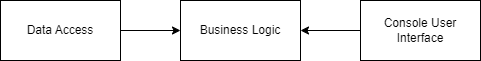
\includegraphics[width=1\textwidth]{shemes/high_arch.drawio.png}
	\caption{Верхеуровневое разбиение на компоненты}
	\label{fig:high_arch}
\end{figure}

\begin{enumerate}
    \item Data Access -- набор классов, представленных паттерном репозиторий, обращающиеся к базе данных;
    \item Business Logic -- набор классов, реализующий логику работы приложения;
    \item Console User Interface -- набор классов, реализующих работу с пользователем, общающиеся далее к слою бизнес-логики.
\end{enumerate}

Слой доступа к данным представлен следующими классами:

\begin{enumerate}
    \item AdminRepository -- управление администраторами;
    \item ClientDynamicRepository -- управление персональными статистиками;
    \item ClientRepository -- управление клиентами;
    \item CoachRepository -- управление тренерами;
    \item CoachScheduleRepository -- управление расписанием тренеров;
    \item EventsRepository -- управление групповыми мероприятиями;
    \item HallRepository -- управление спортивными пространствами;
    \item PersonalTrainingRepository -- управление персональными тренировками;
    \item PersonRepository -- общие методы управления клиентами, тренерами, администраторами.
\end{enumerate}


\section{Выбор системы управления базами данных}

Для анализа были выбраны наиболее распространённые системы управления базами данных, такие как:

\begin{itemize}[label=—]
	\item PostgreSQL \cite{PostgreSQL};
	\item MySQL \cite{MySQL};
	\item SQLite \cite{SQLite};
	\item Microsoft SQL Server \cite{MSSQL}.
\end{itemize}

PostgreSQL -- система управления объектно-реляционной базой данных с открытым исходным кодом и полной поддержкой SQL.
Стабильно получает обновления и является кроссплатформенной. Имеет расширяемую систему встроенных языков программирования,
возможность создавать собственные функции, триггеры, процедуры и индексы. Полностью отвечает требованиям ACID.

В MySQL делается упор на высокую скорость чтения, что делает её незаменимой для создания Web-приложений. 
Однако может быть не так эффективна в отличии от PostgreSQL в сложных аналитических запросах.
MySQL имеет открытый исходный код, работает практически на всех основных платформах. 

SQLite -- компактная встраиваемая система управления базой данных. Имеет ограниченную поддержку SQL синтаксиса,
чаще всего используется в мобильной разработке, десктопных приложениях, браузерах, когда не надо обмениваться данными
с сервером. Среди других особенностей архитектуры можно выделить малый размер памяти, требуемый для установки SQLite, 
и наличие динамической типизации.

Microsoft SQL Server подходит для создания проектов любого размера. Имеет собственный язык запросов 
Transact-SQL и гибкие инструменты администрирования. Однако обладает рядом недостатков, среди которых выделяется
ограниченная совместимость с операционными системами, отличными от Windows, и необходимость выделения больших 
аппаратных ресурсов.

Выбор системы управления базами данных был обусловлен следующими критериями:

\begin{enumerate}
    \item наличие опыта работы;
    \item бесплатное распространение;
    \item наличие подробной документации;
    \item поддержка SQL в достаточном объёме.
\end{enumerate}

В таблице \ref{tab:anal_db} приведены результаты анализа.

\begin{table}[H]
	\centering
	\caption{Результаты анализа существующих конкурентов}
	\begin{tabular}{|c|p{3cm}|p{3cm}|p{2cm}|p{3cm}|}
	\hline
	Номер критерия & PostgreSQL & MySQL & SQLite & 	Microsoft SQL Server \\
	\hline
	1 & + & - & + & - \\
	\hline
	2 & + & + & + & - \\
	\hline
	3 & + & - & + & + \\
	\hline
	4 & + & + & - & + \\
	\hline
	\end{tabular}
	\label{tab:anal_db}
\end{table}

По итогам анализа был выбран PostgreSQL, так как он отвечает всем вышеизложенным критериям.

Сценарии создания базы данных и наложения ограничений приведены в приложениях A и B соответственно.

\section{Классы эквивалентности}

\subsection{Классы эквивалентности для функции get\_coach\_specializations}

Исходные записи в таблицах базы данных представлены в таблицах \ref{tab:coach_db_screen},
\ref{tab:hall_db_screen}, \ref{tab:coachspecialization_db_screen}, \ref{tab:coachspecializationtypes_db_screen}:

\begin{table}[H]
	\centering
	\caption{Записи в таблице coach}
	\begin{tabular}{|c|p{2cm}|p{3cm}|p{2cm}|p{3.5cm}|p{3cm}|}
	\hline
	ID & name & surname & login & password & is\_participate \\
	\hline
	6 & Андрей & Кондукторов & oltpzss4 & пароль в защищённом виде & true \\
	\hline
	7 & Егор & Пучков & egorpuchk & пароль в защищённом виде & true \\
	\hline
	\end{tabular}
	\label{tab:coach_db_screen}
\end{table}

\begin{table}[H]
	\centering
	\caption{Записи в таблице hall}
	\begin{tabular}{|c|p{15cm}|}
	\hline
	ID & name \\
	\hline
	2 & Йога-студия \\
	\hline
	3 & Бассейн \\
	\hline
	1 & Фитнес зал \\
	\hline
	\end{tabular}
	\label{tab:hall_db_screen}
\end{table}

\begin{table}[H]
	\centering
	\caption{Записи в таблице coachspecialization}
	\begin{tabular}{|c|p{7.5cm}|p{7.5cm}|}
	\hline
	ID & specid & coachid \\
	\hline
	1 & 1 & 6 \\
	\hline
	12 & 3 & 6 \\
	\hline
	\end{tabular}
	\label{tab:coachspecialization_db_screen}
\end{table}

\begin{table}[H]
	\centering
	\caption{Записи в таблице coachspecializationtypes}
	\begin{tabular}{|c|p{7.5cm}|p{7.5cm}|}
	\hline
	ID & name & hallid \\
	\hline
	1 & Фитнес & 1 \\
	\hline
	2 & Йога & 2 \\
	\hline
	3 & Бокс & 1 \\
	\hline
	4 & Плавание & 3 \\
	\hline
	\end{tabular}
	\label{tab:coachspecializationtypes_db_screen}
\end{table}

\subsubsection{Класс ввода несуществующего логина тренера}

Вход: oltpzss2

Ожидаемый результат: ничего.

\subsubsection{Класс наличия нескольких специализаций тренера}

Вход: oltpzss4

Ожидаемый результат представлен в таблице \ref{tab:res_class_1}:

\begin{table}[H]
	\centering
	\caption{Результат для класса наличия нескольких специализаций тренера}
	\begin{tabular}{|c|p{7.5cm}|p{7.5cm}|}
	\hline
	ID & Название & Зал проведения \\
	\hline
	1 & Фитнес & Фитнес зал \\
	\hline
	3 & Бокс & Фитнес зал \\
	\hline
	\end{tabular}
	\label{tab:res_class_1}
\end{table}

\subsubsection{Класс отсутствия специализаций у тренера}

Вход: egorpuchk

Ожидаемый результат: ничего.

\subsection{Классы эквивалентности для функции show\_available\_events}

Исходные записи в таблицах базы данных представлены в таблицах \ref{tab:StandartTraining_db_screen},
\ref{tab:trainingsigns_db_screen}:

\begin{table}[H]
	\centering
	\caption{Записи в таблице StandartTraining}
	\begin{tabular}{|c|p{2.7cm}|p{1.6cm}|p{1.6cm}|p{1.2cm}|p{1.6cm}|p{2.5cm}|p{1.6cm}|}
	\hline
	ID & name & adminid & coachid & hallid & capacity & datetime & duration \\
	\hline
	2 & Интенсивный бокс & 2 & 6 & 1 & 10 & 2025-05-01 19:12:28 & 3 \\
	\hline
	1 & Йога & 2 & 6 & 2 & 2 & 2025-06-01 10:48:59 & 1 \\
	\hline
	3 & Растяжка & 2 & 6 & 1 & 15 & 2025-07-29 19:17:36 & 1 \\
	\hline
	\end{tabular}
	\label{tab:StandartTraining_db_screen}
\end{table}

\begin{table}[H]
	\centering
	\caption{Записи в таблице TrainingSigns}
	\begin{tabular}{|c|p{7.5cm}|p{7.5cm}|}
	\hline
	ID & clientid & stdtrainingid \\
	\hline
	1 & 1 & 1 \\
	\hline
	2 & 2 & 1 \\
	\hline
	\end{tabular}
	\label{tab:trainingsigns_db_screen}
\end{table}

\subsubsection{Класс отсутствия доступных тренировок из-за того, что они уже прошли}

Вход: Время, когда клиент обращается к функции: 2025-08-01 10:48:59.

Ожидаемый результат: ничего.

\subsubsection{Класс доступных тренировок, с отсечением прошедших и тех, на которые закончились места}

Вход: Время, когда клиент обращается к функции: 2025-05-30 10:00:00.

Ожидаемый результат представлен в таблице \ref{tab:res_class_2}: 

\begin{table}[H]
	\centering
	\caption{Результат работы функции show\_available\_events}
	\begin{tabular}{|c|p{1.7cm}|p{2cm}|p{2cm}|p{2cm}|p{1.6cm}|p{1.5cm}|p{2.3cm}|}
	\hline
	ID & Назва- ние & Имя тренера & Фамилия тренера & Название зала & Дата & Вмести мость & Продолжи- тельность \\
	\hline
	3 & Растяж- ка & Андрей & Кондук торов & Фитнес зал & 2025-07-29 19:17:36 & 15 & 1 \\
	\hline
	\end{tabular}
	\label{tab:res_class_2}
\end{table}

\subsection{Классы эквивалентности для функции register\_client\_for\_training}

\subsubsection{Класс неуспешной записи из-за идентификатора несуществующего мероприятия}

Вход: идентификатор клиента: 4, идентификатор мероприятия: 150.

Ожидаемый результат: false, 'Тренировка не найдена или уже началась'.

\subsubsection{Класс неуспешной записи из-за отсутствия мест на мероприятие}

Вход: идентификатор клиента: 4, идентификатор мероприятия: 1.

Ожидаемый результат: false, 'Мест на данное мероприятие не осталось'.

\subsubsection{Класс успешной записи на мероприятие}

Вход: идентификатор клиента: 4, идентификатор мероприятия: 3.

Ожидаемый результат: true, 'Вы успешно записаны'.

Новое состояние таблицы TrainingSigns представлено в таблице \ref{tab:new_trainingsigns}.

\begin{table}[H]
	\centering
	\caption{Обновлённая таблица TrainingSigns}
	\begin{tabular}{|c|p{7.5cm}|p{7.5cm}|}
	\hline
	ID & clientid & stdtrainingid \\
	\hline
	1 & 1 & 1 \\
	\hline
	2 & 2 & 1 \\
	\hline
	3 & 4 & 3 \\
	\hline
	\end{tabular}
	\label{tab:new_trainingsigns}
\end{table}

\newpage

\subsubsection{Класс неуспешной повторной записи на мероприятие}

Вход: идентификатор клиента: 4, идентификатор мероприятия: 1.

Ожидаемый результат: false, 'Вы уже записаны на это мероприятие'.

\section{Разработанные функции}

В листингах \ref{lst:client-reg-1} и \ref{lst:client-reg-2} приведена реализация функции регистрации клиента на групповое мероприятие.

\lstinputlisting[
    caption={Функция регистрации клиента на мероприятие. Часть 1},
    label=lst:client-reg-1,
    frame=single,
	linerange={1-25}
]{listings/client_registrate.sql}

\newpage

\lstinputlisting[
    caption={Функция регистрации клиента на мероприятие. Часть 2},
    label=lst:client-reg-2,
    frame=single,
	linerange={27-43}
]{listings/client_registrate.sql}

В листингах \ref{lst:get_coach_specializations-1} и \ref{lst:get_coach_specializations-2} приведена реализация функции получения списка специализаций тренера.

\lstinputlisting[
    caption={Функция получения списка специализаций конкретного тренера. Часть 1},
    label=lst:get_coach_specializations-1,
    frame=single,
	linerange={1-12}
]{listings/get_coach_specializations.sql}

\lstinputlisting[
    caption={Функция получения списка специализаций конкретного тренера. Часть 2},
    label=lst:get_coach_specializations-2,
    frame=single,
	linerange={13-19}
]{listings/get_coach_specializations.sql}

В листингах \ref{lst:show_available_events-1} и \ref{lst:show_available_events-2} приведена реализация функции получения списка доступных групповых мероприятий.

\lstinputlisting[
    caption={Функция получения списка доступных групповых мероприятий. Часть 1},
    label=lst:show_available_events-1,
    frame=single,
	linerange={1-22}
]{listings/show_available_events.sql}
\newpage
\lstinputlisting[
    caption={Функция получения списка доступных групповых мероприятий. Часть 2},
    label=lst:show_available_events-2,
    frame=single,
	linerange={23-33}
]{listings/show_available_events.sql}

\section{Разработанная ролевая модель}

В листингах \ref{lst:roles-1}, \ref{lst:roles-2} и \ref{lst:roles-3} приведена реализация ролевой модели на уровне базы данных.

\lstinputlisting[
    caption={Ролевая модель. Часть 1},
    label=lst:roles-1,
    frame=single,
	linerange={1-11}
]{listings/roles.sql}

\newpage

\lstinputlisting[
    caption={Ролевая модель. Часть 2},
    label=lst:roles-2,
    frame=single,
	linerange={13-48}
]{listings/roles.sql}

\newpage

\lstinputlisting[
    caption={Ролевая модель. Часть 3},
    label=lst:roles-3,
    frame=single,
	linerange={50-83}
]{listings/roles.sql}

\newpage

\section{Демонстрация работы программы}

При запуске пользователя встречает меню с вариантами входа в аккаунт:

\begin{figure}[H]
	\centering
	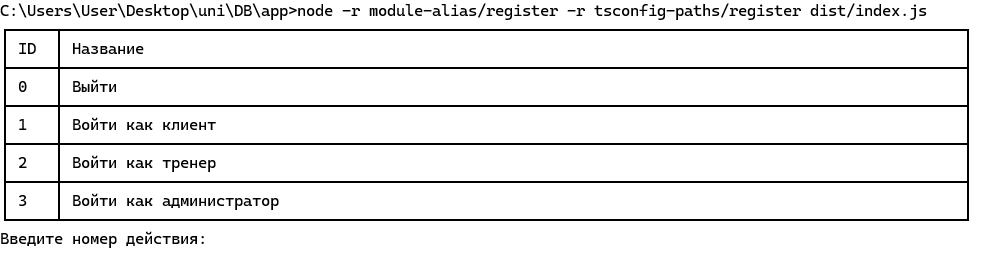
\includegraphics[width=1\textwidth]{img/intro_window.png}
	\caption{Начальное меню приложения}
	\label{fig:intro_window}
\end{figure}

При входе в качестве клиента, пользователю становится доступен следующий набор действий:

\begin{figure}[H]
	\centering
	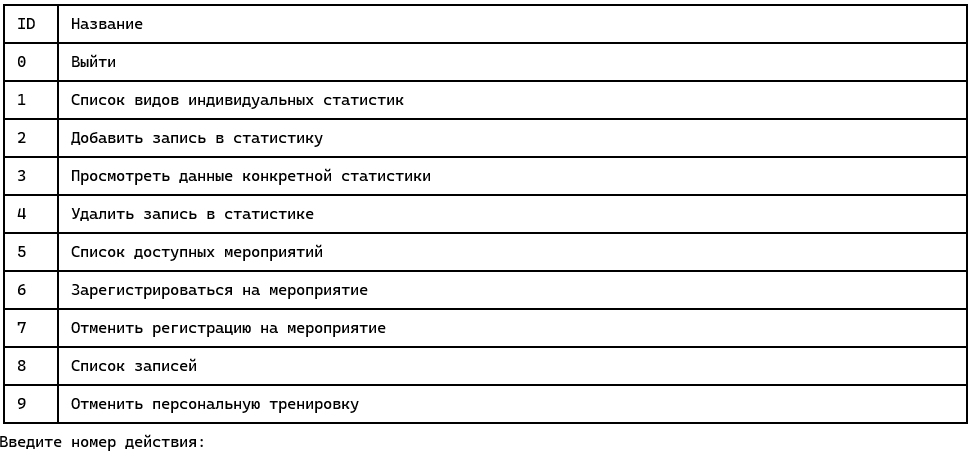
\includegraphics[width=1\textwidth]{img/client_window.png}
	\caption{Меню программы клиента спортивного зала}
	\label{fig:client_window}
\end{figure}

При входе в качестве тренера, пользователю становится доступен следующий набор действий:

\begin{figure}[H]
	\centering
	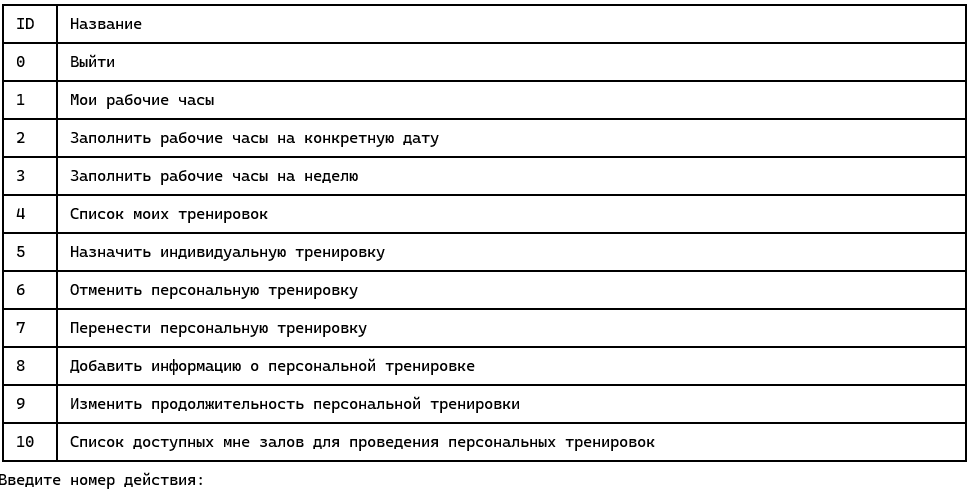
\includegraphics[width=1\textwidth]{img/coach_window.png}
	\caption{Меню программы тренера спортивного зала}
	\label{fig:coach_window}
\end{figure}

При входе в качестве администратора, пользователю становится доступен следующий набор действий:

\begin{figure}[H]
	\centering
	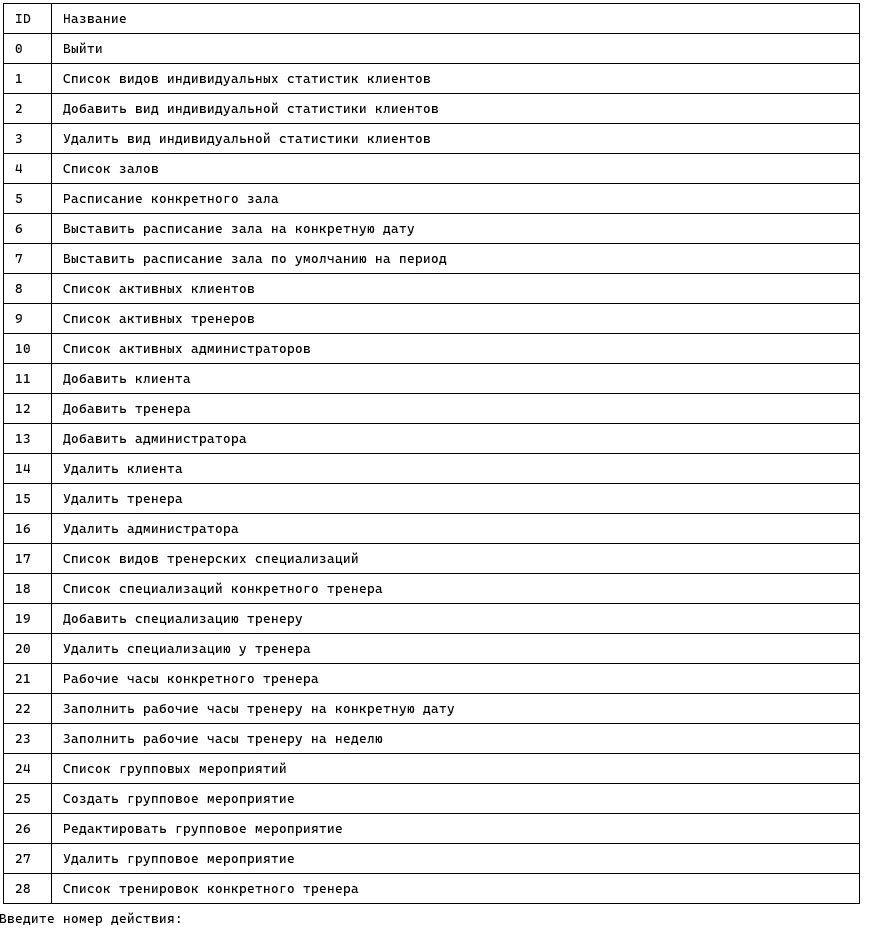
\includegraphics[width=1\textwidth]{img/admin_window.png}
	\caption{Меню программы администратора спортивного зала}
	\label{fig:admin_window}
\end{figure}